\id{МРНТИ 61.61.29}

\begin{articleheader}
\sectionwithauthors{Л.К. Тастанова, А.З. Бекешев, А.С. Мостовой, А.К. Жұмабекова, Г.Д. Серікбаева}{ЭПОКСИДТІ КОМПОЗИТТЕРДІҢ ФИЗИКА-ХИМИЯЛЫҚ ҚАСИЕТТЕРІНЕ
ФУНКЦИОНАЛДЫРЫЛҒАН НАНОТОЛТЫРҒЫШТАРДЫҢ ӘСЕРІ}

{\bfseries \textsuperscript{1}Л.К. Тастанова\textsuperscript{\envelope },
\textsuperscript{1}А.З. Бекешев, \textsuperscript{2}А.С. Мостовой,
\textsuperscript{3}А.К. Жұмабекова, \textsuperscript{1}Г.Д. Серікбаева}
\end{articleheader}

\begin{affiliation}
\textsuperscript{1} Қ.Жұбанов атындағы Ақтөбе өңірлік университеті,
Ақтөбе қ., Қазақстан,

\textsuperscript{2} Ю.Гагарин атындағы Саратов мемлекеттік техникалық
университеті, Саратов қ., Ресей,

\textsuperscript{3} Қ.Құлажанов атындағы Қазақ технология және бизнес
университеті, Астана қ. Қазақстан

\raggedright {\bfseries \textsuperscript{\envelope }}Корреспондент-автор: \href{mailto:lyazzatt@mail.ru}{\nolinkurl{lyazzatt@mail.ru}}
\end{affiliation}

Бұл жұмыста өңделмеген және аминсірке қышқылымен функционалдырылған
наноалмаздар (НА) мен алюминий нитриді (AlN) нанотолтырғыштарының
эпоксидті композиттердің құрылымының қалыптасуына және сипаттамаларына
әсері зерттелді. Сканерлеуші электронды микроскопиялық (СЭМ) талдау осы
нанотолтырғыштардың морфологиясы мен агломерацияға күшті бейімділігін,
яғни олардың дисперстілігін және полимер матрицасымен өзара әрекеттесуін
жақсарту үшін түрлендіру қажеттілігін анықтады. НА және AlN аминсірке
қышқылымен функционализациялау гельдену және қатаю процестерін
айтарлықтай жылдамдатады, бұл термометриялық сонымен қатар
дифференциалдық сканерлеу калориметриясымен өлшенген нәтижелері
көрсетті. Аталған зерттеулер композиттердің қатаю температурасы және
уақытымен қатар оның термиялық эффектісінің жоғарылауын көрсетті.
Механикалық сынақтар аминсірке қышқылымен өңделген НА немесе AlN
нанобөлшектерімен модификацияланған эпоксидті композиттер өңделмеген
нанотолтырғыштар қосылған композиттермен салыстырғанда беріктік,
серпімділік модулі және қаттылық бойынша айтарлықтай жақсартуларды
көрсететінін анықтады. Сонымен қатар, зерттеулер аминсірке қышқылымен
өңделмеген және модификацияланған НА және AlN нанобөлшектерінің қосылуы
эпоксидті нанокомпозиттердің ыстыққа төзімділігі мен термиялық
тұрақтылығын айтарлықтай жақсартатынын көрсетті. Алынған нәтижелер
эпоксидті нанокомпозиттердің физикалық-механикалық қасиеттерін
оңтайландыру үшін аминсірке қышқылымен өңдеудің тиімділігін көрсетті,
бұл заманауи материалдарды дамыту үшін перспективалы жолдарды ашады.

{\bfseries Түйін сөздер:} эпоксидті композит, нанотолтырғыш,
модификациялау, наноалмаздар, алюминий нитриді, аминсірке қышқылы.

\begin{articleheader}
{\bfseries THE EFFECT OF FUNCTIONALIZED NANOFILLERS ON THE PHYSICO-CHEMICAL
PROPERTIES OF EPOXY COMPOSITES}

{\bfseries \textsuperscript{1}L. Tastanova\textsuperscript{\envelope },
\textsuperscript{1}A. Bekeshev, \textsuperscript{2}A. Mostovoy,
\textsuperscript{3}A. Zhumabekova, \textsuperscript{1}G. Serikbayeva}
\end{articleheader}

\begin{affiliation}
\textsuperscript{1}K. Zhubanov Aktobe Regional University, Aktobe,
Kazakhstan,

\textsuperscript{2}Yu. Gagarin State Technical University of Saratov,
Saratov, Russia,

\textsuperscript{3} Kazakh University of Technology and Business,
Astana, Kazakhstan,

е-mail: \href{mailto:lyazzatt@mail.ru}{\nolinkurl{lyazzatt@mail.ru}}
\end{affiliation}

The study explores the impact of incorporating pristine and aminoacetic
acid-functionalized nanofillers, specifically nanodiamonds (ND) and
aluminum nitride (AlN), on the structure formation and performance of
epoxy polymers. Scanning electron microscopy (SEM) analysis reveals the
morphology and pronounced agglomeration tendencies of these nanofillers,
underscoring the need for functionalization to improve their dispersion
and interaction with the polymer matrix. The functionalization of ND and
AlN with aminoacetic acid significantly accelerates the gelation and
curing processes, as evidenced by thermometric and differential scanning
calorimetry (DSC) studies, which show a reduction in curing times and
temperatures along with enhanced thermal effects. Mechanical testing
demonstrates that epoxy composites containing aminoacetic acid-treated
ND and AlN exhibit marked improvements in strength, modulus, and impact
resistance compared to those with pristine nanofillers. Moreover, the
results show that the incorporation of ND and AlN nanoparticles, whether
pristine or aminoacetic acid-modified, notably increases the heat
resistance and thermal stability of epoxy nanocomposites, with higher
aminoacetic acid concentrations correlating with even greater
improvements in these properties. These findings highlight the
effectiveness of aminoacetic acid treatment in optimizing the physical
and mechanical properties of epoxy nanocomposites, offering promising
avenues for advanced material development.

{\bfseries Key words:} epoxy composite, nanofiller, modification;
nanodiamonds, aluminum nitride, aminoacetic acid.

\begin{articleheader}
{\bfseries ВЛИЯНИЕ ФУНКЦИОНАЛИЗИРОВАННЫХ НАНОНАПОЛНИТЕЛЕЙ НА
ФИЗИКО-ХИМИЧЕСКИЕ СВОЙСТВА ЭПОКСИДНЫХ КОМПОЗИТОВ}

{\bfseries \textsuperscript{1}Л. Тастанова\textsuperscript{\envelope },
\textsuperscript{1}А. Бекешев, \textsuperscript{2}А. Мостовой,
\textsuperscript{3}А.К. Жумабекова, \textsuperscript{1}Г.Д. Серикбаева}
\end{articleheader}

\begin{affiliation}
\textsuperscript{1} Актюбинский региональный университет им. К.Жубанова,
г.Актобе, Казахстан,

\textsuperscript{2} Саратовский государственный технический университет
им. Ю.Гагарина, г.Саратов, Россия,

3 Казахский университет технологии и бизнеса им. К.Кулажанова, г.Астана,
Казахстан,

е-mail: \href{mailto:lyazzatt@mail.ru}{\nolinkurl{lyazzatt@mail.ru}}
\end{affiliation}

В работе изучено влияние включения необработанных и
функционализированных аминоуксусной кислотой нанонаполнителей -
наноалмазов (НА) и нитрида алюминия (AlN), на формирование структуры и
характеристики эпоксидных композитов. Анализ методом сканирующей
электронной микроскопии (СЭМ) выявил морфологию этих нанонаполнителей и
выраженную склонность их к агломерации, что подчеркивает необходимость
функционализации для улучшения их дисперсности и взаимодействия с
полимерной матрицей. Функционализация НА и AlN аминоуксусной кислотой
значительно ускоряет процессы гелеобразования и отверждения, о чем
свидетельствуют термометрические исследования и дифференциальная
сканирующая калориметрия (ДСК), которые показывают сокращение времени и
температуры отверждения наряду с усилением теплового эффекта.
Механические испытания показали, что эпоксидные композиты, содержащие НА
и AlN, обработанные аминоуксусной кислотой, демонстрируют заметное
улучшение прочности, модуля упругости и ударной вязкости по сравнению с
композитами с нетронутыми нанонаполнителями. Кроме того, выявлено, что
включение наночастиц НА и AlN, как чистых, так и модифицированных
аминоуксусной кислотой, значительно повышает теплостойкость и
термостабильность эпоксидных нанокомпозитов, причем более высокие
концентрации аминоуксусной кислоты приводят к большему улучшению этих
свойств. Полученные результаты свидетельствуют об эффективности
обработки аминоуксусной кислотой для оптимизации физико-механических
свойств эпоксидных нанокомпозитов, что открывает перспективные пути для
разработки современных материалов.

{\bfseries Ключевые слова:} эпоксидный композит; нанонаполнитель;
модификация; наноалмазы; нитрид алюминия, аминоуксусная кислота.

\begin{multicols}{2}
{\bfseries Кіріспе.} Эпоксидті шайыр негізіндегі композиттер әртүрлі
өнеркәсіптік қолданбаларда жоғары бағаланады, себебі олардың
қасиеттерінің ерекше үйлесімі, соның ішінде жоғары диэлектрлік
сипаттамалары, механикалық беріктігінің жоғарылауы, суға төзімділігі,
агрессивті ортаға төзімділігінің жоғары болуы, минималды тор түзілу
кезіндегі шөгуі және әртүрлі материалдарға күшті адгезиясы байқалады.
Бұл атрибуттар эпоксидті композиттерге минералды байланыстырғыштар мен
полиэфир, фуран және мочевина негізіндегі материалдар сияқты басқа
синтетикалық шайырлардан тұратын дәстүрлі композициялардан асып түсуге
мүмкіндік береді {[}1,2{]}. Бұл композиттерді белгілі бір өнімділік
талаптарына бейімдеу үшін көбінесе пластификаторлар мен толтырғыштар
қосылады. Пластификаторлар полимерлі материалдарға серпімділік береді
және олардың шыныға өту температурасын өзгертеді, ал толтырғыштар
композиттердің механикалық және физика-химиялық қасиеттерін арттырады.

Әртүрлі модификациялаушы қоспалар мен толтырғыштары қосу полимерлі
композиттік материалдардың және олардан алынатын өнімдердің
функционалдық сипаттамаларын жақсартудың кеңінен таралған стратегиясы
болып табылады {[}3-5{]}. Маңызды зерттеу жұмыстары полимерлі матрицаны
әртүрлі минералды толтырғыштармен өзгерту арқылы жаңа эпоксидті
композиттерді жасауға бағытталған {[}6-9{]}. Жиі қолданылатын минералды
ұсақ дисперсті толтырғыштарға тальк, базальт және хромит жатады.
Дегенмен, минералды толтырғыштар мен полимерлі матрицалар арасындағы
адгезияның төмендігіне, сондай-ақ минералды материалдардың агломерацияға
бейімділігіне байланысты қасиеттердің күтілетін жақсаруы жиі күткендей
болмайды.

Эпоксидті матрицаға спецификалық қасиеттері бар нанотолтырғыштарды
енгізу арқылы полимерлі композициялардың наноқұрылымдық сипаттамаларын
бақылау арқылы бейімделген қасиеттері бар композиттерді құру әлеуеті
функционалды полимерлі материалдардың ассортиментін кеңейтудің
перспективалы жолы болып табылады {[}10-12{]}. Бұл тәсіл эпоксидті
шайырлардың сынғыштығы сияқты мәселелерді шешуге мүмкіндік береді,
осылайша берік және бейімделгіш композиттік материалдарды жасауға
мүмкіндік береді. Осы саладағы жүргізіліп жатқан зерттеулер полимерлі
композиттердің жаңа мүмкіндіктерін ашу үшін, әсіресе өнеркәсіптік
талаптарға сәйкес болуы өте маңызды.

Полимерлі нанокомпозиттердің қасиеттерін едәуір арттырудың негізгі
міндеті полимер матрицасында нанобөлшектердің толық дисперсиясына қол
жеткізу болып табылады. Өтпелі немесе трансшекаралық қабат деп аталатын
үлкен фазааралық аймақтың пайда болуы нанобөлшектердің біркелкі таралуын
қиындатады, бұл агрегацияға әкеледі. Бұл композиттік материалдың
біркелкі емес қасиеттеріне және өнімділігінің төмендеуіне әкелуі мүмкін.
Сондықтан нанобөлшектердің біртекті дисперсиясына қол жеткізу
нанокомпозиттік материалдардың артықшылықтарын толық жүзеге асыру үшін
өте маңызды.

Осы мәселені шеше отырып, нанокомпозиттердегі қазіргі зерттеулердің
көпшілігі біркелкі таралуға қол жеткізу және агрегацияның алдын алу үшін
нанобөлшектерді өңдеу мен таратудың тиімді стратегияларын әзірлеуге
бағытталған {[}3-5{]}. Бұл стратегиялар көбінесе матрица мен
нанобөлшектердің өзара әрекеттесуін жақсартуға бағытталған озық
әдістерді қамтиды, осылайша нанокомпозиттің жалпы қасиеттерін
жақсартады.

Нанобөлшектердің агрегациясын азайту және адгезиялық қасиеттерін
жақсарту үшін наноматериалдарды функционализациялау және композиттерді
физикалық түрлендірудің тиімді әдістерін жасау өте маңызды. Толтырғыш
бетін толтырғыш пен полимер матрицасы арасындағы химиялық
әрекеттесулерді жеңілдететін қосылыстармен функционализациялау
толтырғыштың полидисперстілігін төмендетіп, эпоксидті композиттердің
физикалық-механикалық қасиеттерін жақсарта алады {[}13,14{]}. Аминсірке
қышқылы олигомердің эпоксидті топтарымен және нанотолтырғыштармен
әрекеттесетін карбон топтарымен әрекеттесетін амин топтарының арқасында
тиімді функционализациялаушы агент болып шықты.

Полимер матрицасындағы нанотолтырғыштардың тиімді дисперсиясын
қамтамасыз ету полимер байланыстырғыштың едәуір бөлігінің шекаралық
қабатқа, тіпті толтырғыштың төмен концентрациясында (1\%-дан аз) өтуін
жеңілдетуі мүмкін. Мысалы, эпоксидті матрицаға тек 1\% аммиак-су
функционалды графен оксидін қосу композиттің созылу беріктігін де, иілу
беріктігін де екі есе арттыратыны көрсетілген. Сонымен қатар,
композиттің созылу модулі толтырылмаған эпоксидті полимермен
салыстырғанда 1,5 есе өсті, бұл нанотолтырғыштың механикалық
сипаттамасына айтарлықтай әсерін көрсетеді {[}15{]}.

Тағы бір зерттеуде зерттеушілер полимерлі матрицаны полиэфирамин және
алюминий нитридімен (AlN) жұмыс істейтін графеннің кванттық нүктелерімен
өзгерту арқылы композиттің жылу өткізгіштігін арттырды. Осы функционалды
наноматериалдардың 20\% - н қосу жылу өткізгіштіктің бастапқы
өзгертілмеген матрицадан 6,89 есе жоғары мәніне әкелді {[}16{]}. Бұл
нанотолтырғыштардың механикалық қасиеттерін жақсарту үшін ғана емес,
сонымен қатар жылулық сипаттамаларын арттыру үшін де әлеуетін көрсетеді,
бұл материалдарды жылуды тиімді таратуды қажет ететін қолданбалар үшін
қолайлырақ етеді.

Осыған ұқсас жетістіктерге басқа зерттеулерде де қол жеткізілді, мысалы,
AlN және BN гибридті толтырғыштарын пайдалану, ол эпоксидті жабынның
жылу өткізгіштігін 46 есе арттырды, сонымен бірге 22,56 ppm/°c төмен
термиялық кеңею коэффициентін сақтайды {[}17{]}.

Сонымен қатар, наноалмаздар (НА) жоғары беріктігі, жоғары жылу
өткізгіштігі, тамаша оптикалық қасиеттері және биоүйлесімділігі
арқасында матрицаны өзгертетін құнды компонент ретінде пайда болды.
Зерттеулер көрсеткендей, НА функционализациясы композиттік
материалдардың жылу өткізгіштігін де, сынуға төзімділігін де айтарлықтай
жақсарта алады, бұл механикалық сипаттамаларын жақсартуда жақсы
дисперсті наноқұрылымдардың тиімділігін көрсетеді {[}18, 19-20{]}.

Осы жетістіктерге қарамастан, толтырғыштың төменірек концентрациясында
және жергілікті өндірістің үнемді материалдарын пайдалана отырып,
қажетті қасиеттерді жақсарту мәселелері әлі де қалып отыр.
Нанотолтырғыштарды пайдалануды оңтайландыру және өнімділікті жақсартуды
экономикалық және практикалық ойлармен теңестіретін өңдеу әдістерін
әзірлеу үшін қосымша зерттеулер қажет. Зерттелетін тәсілдердің бірі
полимер матрицасымен үйлесімділікті жақсарту және тиімді дисперсияны
қамтамасыз ету үшін нанотолтырғыштарды аминсірке қышқылымен химиялық
модификациялау болып табылады. Нанотолтырғыштардың нақты модификациясына
назар аудара отырып және олардың полимер матрицасымен өзара әрекеттесуін
түсіне отырып, бұл зерттеу алдыңғы зерттеулердің шектеулерін еңсеруге
және жоғары өнімділікті үнемділікпен және өңдеудің қарапайымдылығымен
үйлестіретін композиттік материалдарды әзірлеуге бағытталған.

Осы жұмыста зерттелетін зерттеу бағыттарының бірі аминсірке қышқылымен
химиялық түрлендірілген нанотолтырғыштардың аз мөлшерін енгізу арқылы
эпоксидті шайыр негізіндегі полимерлі матрицаның айтарлықтай нығаюына
қол жеткізуді қамтиды. Нанотолтырғыштардың нақты модификациясына назар
аудара отырып және олардың полимер матрицасымен өзара әрекеттесуін
түсіне отырып, бұл зерттеу алдыңғы зерттеулердің шектеулерін еңсеруге
және жоғары өнімділікті үнемділікпен және өңдеудің қарапайымдылығымен
үйлестіретін композиттік материалдарды әзірлеуге бағытталған. Бұл тәсіл
күштірек және берік қана емес, сонымен қатар қауіпсіз және экологиялық
таза озық материалдарды жасауға мүмкіндік береді.

{\bfseries Материалдар мен әдістер.} ЭД-20 эпоксидті шайыры chimex Limited
(Санкт-Петербург, Ресей) компаниясынан алынды. Амин түріндегі қатайтқыш
- chimex Limited компаниясы шығарған полиэтилен полиамині (ПЭПА).
95-99\% тазалық дәрежесі бар трихлоропропилфосфат -- пластификатор
(ТХПФ) Xuancheng City Trooyawn Refined Chemical Industry Co
Компаниясынан алынды., Ltd. (Қытай).

Бұл зерттеудегі эпоксидті композицияның құрамы эксперименттік сынақтар
арқылы мұқият оңтайландырылды. Эпоксидті олигомердің пластификатор мен
қатайтқышқа қатынасы салмағы бойынша 100 бөлік (м.ү.) ЭД-20, 40 м.ү.
ТХПФ және 15 м.ү. ПЭПА {[}21,22{]}. Бұл нақты тұжырым композицияның
механикалық беріктіктің, термиялық тұрақтылықтың және отқа төзімділіктің
қажетті тепе-теңдігін көрсетуін қамтамасыз етеді.

Наноалмаздар (НА) және алюминий нитридтері (AlN) құрылымды өзгертетін
бірегей әсерлерін пайдалану үшін салмағы бойынша 1\%-ға дейін аз
мөлшерде қосылды.

Нанотолтырғыштар мен эпоксидті матрица арасындағы өзара әрекеттесуді
одан әрі күшейту үшін толтырғыш нанобөлшектерінің беті аминсірке
қышқылының (АСҚ) көмегімен функционалдандырылды (VitaReactiv LLC,
Дзержинск, Ресей). Наноалмаздар мен алюминий нитридінің беті аминсірке
қышқылымен өңделген. Осы мақсатта ультрадыбыстық гомогенизатордың
көмегімен 50 мл Н2О-аминсірке қышқылының ерітіндісінде 15 минут ішінде
0,25 г тиісті толтырғыш дисперсті болды; аминсірке қышқылының
концентрациясы 2,5\%, 5,0\%, 7,5\% және 10,0\% құрады. Содан кейін
суспензияны 12 сағат бойы 100 айн/мин жылдамдықпен тұрақты төмен
жылдамдықта араластыра отырып 80℃ температурада рефлюкске ұшырады.
Нанотолтырғыш бөлшектерінің айналасындағы артық аминсірке қышқылын
кетіру үшін суспензия центрифугадан өткізіліп, тазартылған сумен екі рет
жуылды. Содан кейін алынған өнім 80 ℃ температурада 5 сағат кептірілді.

Таралу біркелкілігін арттыру және НА және AlN бөлшектерінің агрегациясын
болдырмау, сондай-ақ олардың беті мен байланыстырғышын белсендіру үшін
композицияны ультрадыбыстық өңдеу қолданылды. Ультрадыбыстық өңдеу
параметрлері: жиілігі-22±2 кГц, қуаты - 400 Вт, ұзақтығы - 60 мин. Қоспа
вакуумда 25 ± 5 °C температурада 30 минут ішінде газсыздандырылды.

НА және AlN бөлшектерінің морфологиясы Tescan Vega 3 SBH сканерлеуші
электронды микроскоптың көмегімен зерттелді (Брно, Чехия).

Созылу және иілу беріктігін анықтау үшін Time Group Inc компаниясы
шығарған WDW-5Е сынақ машинасы пайдаланылды (Пекин, Қытай). Созылудың
беріктік шегі және иілудің серпімділік модулін анықтау үшін үлгілер
сәйкесінше 5 және 50 мм/мин жылдамдығымен сыналды. Иілу кезіндегі созылу
беріктігі мен иілу кезіндегі серпімділік модулін анықтау үшін үлгілер
{[}23{]} бойынша сыналды, сынақтар қалыңдығы 4 мм, ені 10 мм және жұмыс
ұзындығы 80 мм блоктар түріндегі үлгілерде жүргізілді. Созылу
беріктігінің шегі мен созылудың серпімділік модулін анықтау үшін үлгілер
{[}24{]} сәйкес сыналды, сынақтар қалыңдығы 4 мм, ені 10 мм және жұмыс
бөлігінің ұзындығы 50 мм шпатель түріндегі үлгілерде жүргізілді. Соққыға
төзімділігін анықтау үшін {[}25{]} сәйкес LCT-50D сынақ стенді (Beijing
United Test Co., ltd.)., Ltd., Пекин, Қытай) пайдаланылды.

Вик бойынша жылуға төзімділікті {[}26{]} әдісіне сәйкес анықтады, В50
әдісі -- жүктеме 50 Н; температураның көтерілу жылдамдығы 50 ℃/сағ.
Термогравиметриялық талдау Q-1500D дериватографында (Будапешт, Венгрия)
жүргізілді. Салмағы 100 мг үлгілер 10℃/мин жылдамдықпен 800℃ дейін
қыздырылды. Талдау ауада жүргізілді және салыстырмалы қателік 1\% - дан
аспады. Бұл талдауда үлгілерді қыздыру кезінде массаның өзгеруі,
массаның өзгеру жылдамдығы және жылу эффектілері зерттелді.

Қатайту процестерінің кинетикасын дифференциалды сканерлеуші
калориметрия (ДСК) әдісімен «ДТАС-1300» құралында келесі шарттарда
зерттелді: сынама массасы - 20 мг, қыздыру аралығы - 400°С дейін,
қыздыру жылдамдығы - минутына 16 градус. ДСК әдісінен басқа, G = f (τ,
T) тәуелділігін сызу арқылы құрылымның қалыптасу процестерін зерттеу
үшін термометриялық әдіс қолданылды, мұндағы τ-процестің ұзақтығы (м);
T-температура (С). Бұл талдауда объектілердің жылудан оқшаулануы
қамтамасыз етілді. Бұл жылу берудің қатаю процесіне әсерін зерттеуге
мүмкіндік берді.

Эпоксидті нанокомпозиттерді сынау келесі әдістерді қолдану арқылы
жүргізілді:

\begin{itemize}
\item
  иілу кезіндегі иілу кернеуін және серпімділік модулін анықтау
  {[}27{]},
\item
  созылу кезіндегі беріктік шегі және серпімділік модулін анықтау
  {[}24{]};
\item
  соққыға төзімділікті анықтау {[}25{]};
\item
  Вик бойынша жылуға төзімділігін анықтау {[}26{]};
\item
  жылу өткізгіштік пен жылу кедергісін анықтау ITP-MG4 "100"
  құрылғысында жүргізілді {[}28{]};
\item
  эпоксидті құрамның қатаю кинетикасын анықтау {[}29{]} сипатталған әдіс
  бойынша жүргізілді.
\end{itemize}

{\bfseries Нәтижелер және талқылау.} Наноалмаз және алюминий нитридінің SEM
кескіндері 1-суретте көрсетілген. Наноалмаз бөлшектері сфералық
морфологияны көрсетеді (1а-сурет). Құрылымдық жағынан бұл бөлшектер
көміртегі құрамдас бөлігі ретсіз көміртегі қабығымен қоршалған алмаз
өзегінен тұратын алып молекулаларға ұқсайды. Бұл қабық одан әрі беткі
көміртегі атомдарының компенсацияланбаған валенттіліктерінде
локализацияланған беттік функционалды топтармен байланысты.
Наноалмаздардың беткі қабатындағы полярлық топтардың көптігі олардың
күрделі коллоидты-химиялық қасиеттеріне ықпал етіп, бөлшектердің едәуір
агломерациясына әкеледі. Бұл агломерация 500-ден 1000 нм-ге дейінгі
өлшемдегі, ал жеке бөлшектердің өзі 10-50 нм наноөлшемді диапазонда
қалады. AlN бөлшектері (1b-сурет) өлшемі 500-ден 2000 нм-ге дейінгі
үлкен агрегаттар түрінде пайда болады, олар өлшемдері 100-ден 300 нм-ге
дейінгі қабыршақ тәрізді ұсақ бөлшектерден тұрады. Бұл ұсақ бөлшектер
олардың дұрыс емес пішінді жиектерімен сипатталады.

Зерттелетін наноматериалдар бөлшектерінің өлшемдері мен құрылымын талдау
агломерацияға айқын бейімділікті анықтады, бұл осы бөлшектерді қамтитын
полимерлі композиттердің беріктік сипаттамаларының минималды
жоғарылауына әкелуі мүмкін. Бұл нәтижелер агломерацияны азайту және
полимер матрицасы/нанобөлшек шекарасында химиялық әрекеттесулерді
күшейту үшін нанобөлшектерді функционализациялаудың маңыздылығын
көрсетеді.
\end{multicols}

\begin{figure}[H]
	\centering
	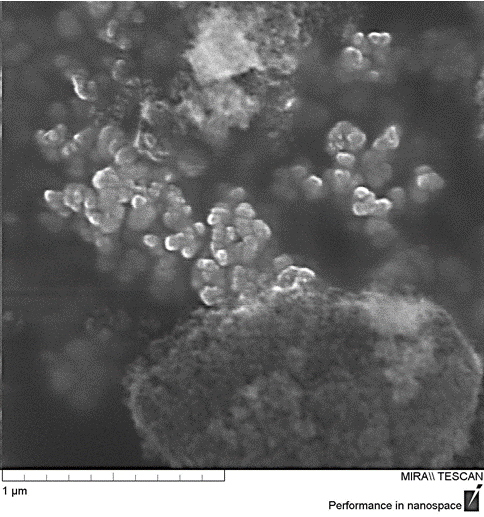
\includegraphics[width=0.8\textwidth]{media/chem/image17}
	\caption*{}
\end{figure}

\begin{figure}[H]
	\centering
	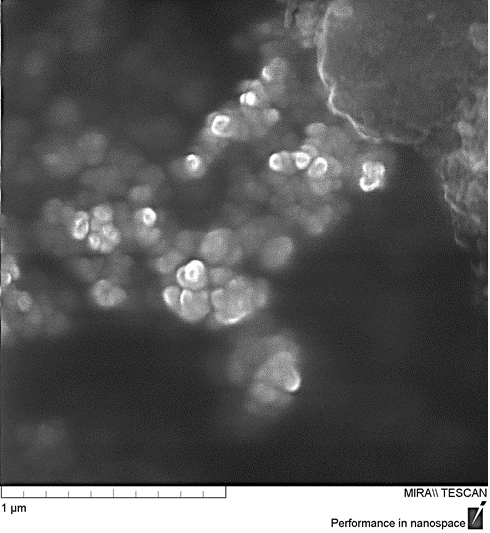
\includegraphics[width=0.8\textwidth]{media/chem/image18}
	\caption*{}
\end{figure}


a б

{\bfseries 1-сурет. Наноалмаз (а) және алюминий нитридінің (б)
бөлшектерінің СЭМ бейнелері. 100~000 есе үлкейтілген}

Модификациялайтын қоспалардың торлы полимерлерге әсерін бағалау кезінде
қатаю процесі наноалмаздар (НА) және алюминий нитридтері (AlN) сияқты
қатты материалдардың дамыған беті болған кезде жүретінін ескеру қажет.
Бұл қатты беттер қатаю кезінде полимерлену реакциясының кинетикалық
сипаттамаларына, сондай-ақ материалдың фазалық құрылымының қалыптасуына
айтарлықтай әсер етуі мүмкін. Бұл процестерде олигомерлі компоненттер
мен НА және AlN -нің қатты беттері арасындағы адсорбциялық өзара
әрекеттесу шешуші рөл атқарады. Қатаю кезінде құрылымның түзілуіне таза
және модификацияланған НА және AlN-нің әсері байқалды (2-сурет).

Эпоксидті құрамға таза НА қосу полимерлену процесін жылдамдатуға әкелді,
бұл гельдену уақытының 104-тен 95 минутқа дейін (2а-сурет) және қатаю
уақыты 146-дан 142 минутқа дейін (2b-сурет) қысқаруымен, сонымен қатар
өздігінен қызудың максималды температурасының 88-ден 110°C-қа дейін
жоғарылауымен дәлелденді (2с-сурет). Полимерленудің бұлай үдетілуі
жылудың көбірек бөлінуімен бірге, полимерлену процесіне НА белсенді
қатысатынын болжауға мүмкіндік береді. Сонымен қатар, эпоксидті құрамға
аминсірке қышқылымен функционалданған НА енгізілгенде, реакцияға
қабілетті амин топтарының қатысуына байланысты полимерлеу процесі одан
әрі жеделдетілді. Бұл гельдену уақытының 78-82 минутқа дейін қысқаруына
және қатаю уақытының 106-114 минутқа дейін қысқаруына әкелді, өздігінен
қызудың максималды температурасы 115-122°C дейін көтерілді (2а-с
суреттер).

а

б

с

{\bfseries 2 - сурет. Эпоксидті композициялардың қатаю процесінің
сипаттамалары: а-гельдену уақыты, в-қатаю уақыты, с-қатаю кезінде
үлгінің өздігінен қызуының максималды температурасы:}

\emph{1 -- ЭД-20 + ТХПФ + ПЭПА,}

\emph{2 -- ЭД-20 + ТХПФ + өңделмеген толтырғыш + ПЭПА,}

\emph{3 - ЭД-20 + ТХПФ + толтырғыш (2.5\% аминсірке қышқылы) + ПЭПА,}

\emph{4 - ЭД-20 + ТХПФ + толтырғыш (5.0\% аминсірке қышқылы) + ПЭПА,}

\emph{5 - ЭД-20 + ТХПФ + толтырғыш (7.5\% аминсірке қышқылы) + ПЭПА}

Осы сияқты, эпоксидті құрамға таза AlN енгізу полимерлеу процесін
тездетіп, гельдену уақытын 104-тен 75 минутқа дейін (2а-Сурет) және
қатаю уақытын 146-дан 105 минутқа дейін (2b-сурет) қысқартты, сонымен
бірге өздігінен қызудың максималды температурасын 88-ден 105°C-қа дейін
жоғарылатты (2с-сурет). Аминсірке қышқылымен функционалдандырылған AlN
қосылған кезде полимерлеу процесі одан әрі жетілдірілді, бұл гельдену
уақытының 53-70 минутқа дейін және қатаю уақытының 79-97 минутқа дейін
қысқаруымен және максималды өздігінен қыздыру температурасы 120-128°С
дейін көтерілуімен қатар жүрді (2а-с суреттер).

Алынған деректерді талдау құрамында модификацияланған НА және AlN бар
эпоксидті композиттердегі амин сірке қышқылы концентрациясының
жоғарылауы құрылымның түзілу процесін жеделдететінін көрсетеді, бұл
тиімдірек қатаюға және термиялық қасиеттердің жақсаруына әкеледі.

а

б

{\bfseries 3 - сурет. Наноалмазбен модификацияланған эпоксидті
композиттердің қатаю процесінің сипаттамалары: а) қатаю процесінің
басталу температурасы (Т\textsubscript{б}), аяқталу температурасы
(Т\textsubscript{а}) және қатаю кезінде максималды жылу шығару
температурасы (T\textsubscript{макс}); б) реакция энтальпиясы}

Эпоксидті композиттердің қатаю кинетикасын термометриялық әдістерді
қолдана отырып зерттеу нәтижесінде алынған мәліметтер негізінде бастапқы
және модификацияланған наноалмаздар мен алюминий нитридінің қатаю
кезінде құрылым түзілуіне әсері анықталды. Эпоксидті матрицаға аминсірке
қышқылымен функционалдандырылған нанобөлшектерді қосу полимерлеу
процесін едәуір жылдамдатады. Бұл жеделдету полимерлену реакциясына
реакцияға қабілетті амин топтарының қатысуына байланысты гельдену уақыты
мен қатаю уақытының қысқаруымен түсіндіріледі. Сонымен қатар,
композициялардың өзін-өзі қыздыруының максималды температурасының
жоғарылауы байқалды (3,4-суреттер).

a

б

{\bfseries 4-сурет. AlN-мен модификацияланған эпоксидті композиттердің
қатаю процесінің сипаттамалары: а) қатаю процесінің басталу
(Т\textsubscript{б}), аяқталу (Т\textsubscript{а}) температуралары және
қатаю кезінде максималды жылу шығару температурасы
(T\textsubscript{макс}); б) реакция энтальпиясы}

Деректерді одан әрі талдау аминсірке қышқылы концентрациясының
жоғарылауы модификацияланған нанобөлшектері бар эпоксидті
композиттердегі құрылымның түзілу жылдамдығын арттыратынын көрсетеді.
Бұл нәтижелер дифференциалды сканерлеу калориметриясымен расталады, бұл
эпоксидті құрамға аминсірке қышқылымен өңделген наноалмаздарды енгізу
қатаю реакциясының энтальпиясын 488 Дж/г-ден 588-691 Дж/г диапазонына
дейін арттыратынын көрсетеді. Энтальпияның бұл жоғарылауы, қатаюдың
басталу температурасының 66°С-тан 41-64°С-қа дейін төмендеуімен бірге
(3-суретте көрсетілгендей), функционалданған нанобөлшектермен
жеңілдетілген қатаю процесінің басталуы мен жеделдеуін растайды.

Эпоксидті құрамға аминсірке қышқылымен өңделген алюминий нитридінің
қосылуы қатаю реакциясының энтальпиясын 660 Дж/г-ден 671-700 Дж/г
диапазонға дейін айтарлықтай жоғарылатуға алып келеді. Бұл модификация
сонымен қатар қатаю процесін тиімдірек бастайды, бұл қатаюдың басталу
температурасының 57°С-тан 43-52°С диапазонына дейін төмендеуімен
дәлелденеді (4-суретті қараңыз).

Дифференциалды сканерлеу калориметриясын қолдана отырып, эпоксидті
композициялар бойынша зерттеу нәтижелерін талдау эпоксидті құрамға
аминсірке қышқылымен жұмыс істейтін нанобөлшектерді қосу полимерлеу
процесін күшейтетінін көрсетеді. Бұл полимерлену реакциясына реакцияға
қабілетті амин топтарының қатысуына байланысты, және ол қатаюдың
бастапқы температурасының төмендеуіне әкеледі. Сонымен қатар,
полимерлену реакциясының жылулық әсерінің жоғарылауы байқалады.
Сондай-ақ, аминсірке қышқылының жоғары концентрациясы модификацияланған
нанобөлшектері бар эпоксидті композиттер құрылымының түзілуін тездетеді.

5 және 6-суреттерде наноалмаз (НА) және алюминий нитридінің (AlN)
бөлшектері бар эпоксидті нанокомпозиттердің деформациялық және беріктік
сипаттамалары көрсетілген.

{\bfseries 5-сурет. Эпоксидті композиттердің қасиеттері: 1-ЭД-20+ТХПФ+ПЭПА;
2-ЭД-20+ТХПФ+НА + ПЭПА; 3 - ЭД-20+ТХПФ+НА (аминсірке}
{\bfseries қышқылы)+ПЭПА}

Эпоксидті матрицаға НА қосу оның механикалық қасиеттерін айтарлықтай
жақсартады. Иілу беріктігі бастапқы эпоксидті полимердегі 85 МПа-дан 110
МПа-ға дейін, серпімділік модулінің 2077 МПа-дан 3676 МПа-ға дейін
айтарлықтай өсуімен бірге жүреді. Сонымен қатар, созылу беріктігі 34
МПа-дан 52 МПа-ға дейін көтеріледі, сәйкесінше созылу кезіндегі
серпімділік модулінің 1634 МПа-дан 2220 МПа-ға дейін жоғарылауы
байқалады. Бір қызығы, эпоксидті полимерлер үшін маңызды болып табылатын
соққыға төзімділік те жақсарады, соққы күші 9
кДж/м\textsuperscript{2}-ден 14 кДж/м\textsuperscript{2}-ге дейін артады
(5-сурет). Соққыға төзімділіктің бұл жоғарылауы эпоксидті композиттердің
сынғыштығын ескере отырып, олардың дәстүрлі түрде қолданылуын шектейді.

Сонымен қатар, эпоксидті композицияға аминсірке қышқылымен өңделген НА
қосу композиттің тасымалдау сипаттамаларын одан әрі арттырады. Бұл өңдеу
иілу беріктігінің 132 МПа-ға дейін айтарлықтай артуына әкеліп соғады, ал
иілу кезінде серпімділік модулі 4199 МПа-ға дейін артады. Созылу
беріктігі де 62 МПа-ға дейін артады, созылу кезіндегі серпімділік модулі
2400 МПа-ға жетеді, ал соққыға төзімділік 17,2
кДж/м\textsuperscript{2}-ге дейін айтарлықтай жақсарады.

{\bfseries 6-сурет. Эпоксидті композиттердің қасиеттері: 1 - ЭД-20 + ТХПФ +
ПЭПА;}

{\bfseries 2 - ЭД-20 + ТХПФ + AlN + ПЭПА; 3 - ЭД-20 + ТХПФ + AlN(аминсірке}
{\bfseries қышқылы) + ПЭПА}

6-суретте алюминий нитриді (AlN) қосылған эпоксидті нанокомпозиттер үшін
ұқсас мәліметтер келтірілген. AlN енгізу композиттің механикалық
қасиеттерін жақсартады. Иілу беріктігі бастапқы эпоксидті полимердегі 85
МПа-дан 96 МПа-ға дейін артады, ал серпімділік модулі 2077 МПа-дан 3286
МПа-ға дейін артады. Созылу беріктігі де 34 МПа-дан 53 МПа-ға дейін
жақсарады, созылу кезіндегі серпімділік модулі 1634 МПА-дан 2091 МПА-ға
дейін артады. Соққы күші 9 кДж/м\textsuperscript{2}-ден 14
кДж/м\textsuperscript{2}-ге дейін айтарлықтай артады.

AlN-н аминсірке қышқылымен өңдеп, эпоксидті құрамға қосқанда, алынған
нанокомпозиттер жоғары механикалық қасиеттерді көрсетеді. Атап айтқанда,
иілу беріктігі 115 МПа-ға дейін артады, иілу кезінде серпімділік модулі
3732 МПа-ға дейін көтеріледі, созылу беріктігі 60 МПа-ға жетеді, созылу
кезіндегі серпімділік модулі 2230 МПА-ға дейін артады, ал соққы
беріктігі 21,0 кДж/м\textsuperscript{2}-ге дейін артады.

Нанобөлшектердің құрылымдық әсері қоспалардың шағын деңгейлерінде де
айқын көрінеді. Полимерлер табиғаты бойынша микрогетерогенді болып
табылады, олардың құрамында тығыз оралған, реттелген аймақтар да, әлсіз,
ақаулы аймақтар да бар. Наномодификаторлар осы ақаулы аймақтарда
локализациялануға бейім, олар маңызды құрылымды-модификациялаушы рөл
атқаруы мүмкін. Бұл локализация полимер тізбектерінің қозғалғыштығын
арттыра отырып, полимердің кинетикалық ынталандырылған реттелуіне ықпал
етеді және тығыз орауға мүмкіндік береді.

Энергетикалық тұрғыдан алғанда, эпоксидті композиттерді нанобөлшектерді
(НА және AlN) енгізу арқылы күшейту материалды жоюға қажетті энергияның
жоғарылауымен түсіндіріледі. Энергияның бұл ұлғаюы жарықшақтың
айналасындағы нанобөлшектер ағынымен және жарықшақ фронтының ұзаруына
байланысты жарықшақ жолының бойында жаңа беттің пайда болуымен
байланысты.

Нанобөлшектердің әртүрлі концентрацияларының әсерінің жиынтық
нәтижелері, сондай-ақ аминқышқылының әртүрлі концентрацияларымен
функционалданған нанобөлшектердің эпоксидті нанокомпозиттердің жылулық
төзімділігіне әсері 1-кестеде көрсетілген.

{\bfseries 1-кесте. Нанобөлшектердің және аминқышқылының әртүрлі
концентрацияларының эпоксидті нанокомпозиттердің жылулық төзімділігіне
әсері}

% \begin{longtable}[]{@{}
%   >{\raggedright\arraybackslash}p{(\columnwidth - 2\tabcolsep) * \real{0.7113}}
%   >{\raggedright\arraybackslash}p{(\columnwidth - 2\tabcolsep) * \real{0.2887}}@{}}
% \toprule\noalign{}
% \begin{minipage}[b]{\linewidth}\raggedright
% {\bfseries Композит құрамы, м.ү.,} (15 м.ү. ПЭПА қатайтылған)
% \end{minipage} & \begin{minipage}[b]{\linewidth}\raggedright
% Жылуға төзімділік температурасы, \textsuperscript{о}С
% \end{minipage} \\
% \midrule\noalign{}
% \endhead
% \bottomrule\noalign{}
% \endlastfoot
% 100ЭД-20 + 40ТХПФ & 110 \\
% \multicolumn{2}{@{}>{\raggedright\arraybackslash}p{(\columnwidth - 2\tabcolsep) * \real{1.0000} + 2\tabcolsep}@{}}{%
% НА мен модификацияланған эпоксидты құрамдар} \\
% 100ЭД-20 + 40ТХПФ + 0,01НА & 132 \\
% 100ЭД-20 + 40ТХПФ + 0,05НА & 136 \\
% 100ЭД-20 + 40ТХПФ + 0,10НА & 142 \\
% 100ЭД-20 + 40ТХПФ + 0,50НА & 146 \\
% 100ЭД-20 + 40ТХПФ + 0,1НА (2,5\% аминсірке қышқылы) & 146 \\
% 100ЭД-20 + 40ТХПФ + 0,1НА (5,0\% аминсірке қышқылы) & 156 \\
% 100ЭД-20 + 40ТХПФ + 0,1НА (7,5\% аминсірке қышқылы) & 166 \\
% \multicolumn{2}{@{}>{\raggedright\arraybackslash}p{(\columnwidth - 2\tabcolsep) * \real{1.0000} + 2\tabcolsep}@{}}{%
% AlN мен модификацияланған эпоксидты құрамдар} \\
% 100ЭД-20 + 40ТХПФ + 0,01AlN & 148 \\
% 100ЭД-20 + 40ТХПФ + 0,05AlN & 152 \\
% 100ЭД-20 + 40ТХПФ + 0,1AlN & 154 \\
% 100ЭД-20 + 40ТХПФ + 0,5AlN & 168 \\
% 100ЭД-20 + 40ТХПФ + 0,05 AlN (2,5\% аминсірке қышқылы) & 160 \\
% 100ЭД-20 + 40ТХПФ + 0,05 AlN (5,0\% аминсірке қышқылы) & 174 \\
% 100ЭД-20 + 40ТХПФ + 0,05 AlN (7,5\% аминсірке қышқылы) & 182 \\
% \end{longtable}

\begin{multicols}{2}
Эпоксидті құрамға 0,01-ден 0,5 Вт-қа дейінгі мөлшерде таза
наноалмаздарды енгізу эпоксидті композиттің ыстыққа төзімділігін
110°C-тан 132-146°C-қа дейін арттыруды қамтамасыз етеді. Сонымен қатар,
аминсірке қышқылымен өңделген наноалмаздарды қосу эпоксидті композиттің
ыстыққа төзімділігін тиімдірек арттыруды қамтамасыз етеді, ал
наноалмаздарды өңдеу үшін қолданылатын аминсірке қышқылының
концентрациясы неғұрлым жоғары болса, эпоксидті нанокомпозиттің ыстыққа
төзімділігі соғұрлым жоғары болады. Аминсірке қышқылының концентрациясын
2,5\% - дан 7,5\% - ға дейін арттыру құрамында 0,1м.ү. НА бар эпоксидті
композицияның ыстыққа төзімділігін 142°C-тан 146-166°c-қа дейін
арттыруды қамтамасыз етеді, (1-кесте).

Эпоксидті құрамға 0,01-ден 0,5 м.ү.-ке дейінгі мөлшерде таза AlN енгізу
эпоксидті композиттің ыстыққа төзімділігін 110 ° C-тан 148-168 ° C-қа
дейін арттырады. Сонымен қатар, AlN өңдеу үшін қолданылатын аминсірке
қышқылының концентрациясы неғұрлым жоғары болса, эпоксидті
нанокомпозиттің ыстыққа төзімділігі соғұрлым жоғары болады. Осылайша,
аминсірке қышқылының концентрациясын 2,5\% - дан 7,5\% - ға дейін
арттыру құрамында 0,05 м.ү. AlN бар эпоксидті композиттің ыстыққа
төзімділігін 152 \textsuperscript{0}С-тан 160-182
\textsuperscript{0}С-қа дейін арттыруды қамтамасыз етеді (1-кесте).

Эпоксидті нанокомпозиттердің термиялық тұрақтылығы термогравиметриялық
талдау әдісімен зерттелді. Алынған мәліметтер 2-кестеде келтірілген.
\end{multicols}

{\bfseries 2-кесте. Эпоксидті нанокомпозиттерді термогравиметриялық зерттеу
нәтижелері}

% \begin{longtable}[]{@{}
%   >{\raggedright\arraybackslash}p{(\columnwidth - 10\tabcolsep) * \real{0.4474}}
%   >{\raggedright\arraybackslash}p{(\columnwidth - 10\tabcolsep) * \real{0.0755}}
%   >{\raggedright\arraybackslash}p{(\columnwidth - 10\tabcolsep) * \real{0.0897}}
%   >{\raggedright\arraybackslash}p{(\columnwidth - 10\tabcolsep) * \real{0.0898}}
%   >{\raggedright\arraybackslash}p{(\columnwidth - 10\tabcolsep) * \real{0.0983}}
%   >{\raggedright\arraybackslash}p{(\columnwidth - 10\tabcolsep) * \real{0.1993}}@{}}
% \toprule\noalign{}
% \begin{minipage}[b]{\linewidth}\raggedright
% {\bfseries Композит құрамы, м.ү.,} (15 м.ү. ПЭПА қатайтылған)
% \end{minipage} & \begin{minipage}[b]{\linewidth}\raggedright
% T\textsubscript{5\%},
% 
% °C
% \end{minipage} & \begin{minipage}[b]{\linewidth}\raggedright
% T\textsubscript{30\%},
% 
% °C
% \end{minipage} & \begin{minipage}[b]{\linewidth}\raggedright
% T\textsubscript{50\%},
% 
% °C
% \end{minipage} & \begin{minipage}[b]{\linewidth}\raggedright
% T\textsubscript{70\%},
% 
% °C
% \end{minipage} & \begin{minipage}[b]{\linewidth}\raggedright
% 800 °C температурадағы қалдық, салмағы \%
% \end{minipage} \\
% \midrule\noalign{}
% \endhead
% \bottomrule\noalign{}
% \endlastfoot
% 100ЭД-20 + 40ТХПФ & 190 & 279 & 385 & 515 & 5.10 \\
% 100ЭД-20 + 40ТХПФ + 0.10НА & 205 & 284 & 394 & 525 & 3.70 \\
% 100ЭД-20 + 40ТХПФ + 0,1НА
% 
% (5.0\% аминсірке қышқылы) & 216 & 291 & 412 & 536 & 5.20 \\
% 100ЭД-20 + 40ТХПФ + 0.05AlN & 200 & 281 & 392 & 518 & 4.85 \\
% 100ЭД-20 + 40ТХПФ + 0.05AlN
% 
% (5.0\% аминсірке қышқылы) & 214 & 290 & 410 & 534 & 5.51 \\
% \end{longtable}

\emph{Ескерту: T\textsubscript{5\%}, T\textsubscript{30\%},
T\textsubscript{50\%} және T\textsubscript{70\%} сәйкесінше 5\%, 30\%,
50\%, 70\% масса жоғалту кезіндегі температуралар.}

\begin{multicols}{2}
Алынған деректерді талдау көрсеткендей, аминсірке қышқылымен
функционалданған наноалмаз бөлшектері мен алюминий нитридін енгізу
эпоксидті композиттің ыдырауының бастапқы температурасының жоғарылауын
қамтамасыз етеді, бұл t5\% индексінің сәйкесінше 190°C-тан 216°C-қа
дейін және 190°C-тан 214°C-қа дейін жоғарылауымен расталады. Сонымен
қатар, эпоксидті композитке аминсірке қышқылымен өңделген НА және AlN
қосылуы эпоксидті нанокомпозиттердің термиялық тұрақтылығын арттыратыны
анықталды, бұл T30\%, T50\% және T70\% жоғарылауымен расталады
(2-кесте). НА және AlN енгізу 800°C температурада көміртегі
қалдықтарының айтарлықтай өсуіне әкелмейтіні анықталды.

{\bfseries Қорытынды.} Бұл зерттеу таза және модификацияланған
нанотолтырғыштардың, атап айтқанда алюминий нитриді (AlN) мен
наноалмаздардың (НА) эпоксидті композит құрылымының қалыптасу
процестеріне айтарлықтай әсер ететінін және гельдену мен қатаю уақытын
дәл реттеуге мүмкіндік беретінін көрсетеді. Нанобөлшектердің беттерін
функционализациялау, әсіресе аминсірке қышқылымен (глицин) өңдеу, қатаю
процестерінің тиімдірек басталуына ықпал етеді, бұл гельдену мен
полимерлену уақытын қысқартады және жылулық әсерлерді арттырады.
Дифференциалды сканерлеу калориметриясы (DSC) бойынша жүргізілген
зерттеулер аминсірке қышқылымен функционалданған нанобөлшектерді
эпоксидті матрицаға енгізу амин топтарының реакциялық қабілеттілігінің
арқасында полимерлену процесін жеделдетіп қана қоймай, сонымен қатар
полимерленудің жылулық әсерін күшейте отырып, қатаюдың бастапқы
температурасын төмендететінін көрсетті.

Алынған эпоксидті композиттердің механикалық қасиеттері аминсірке
қышқылымен өңделген наноалмаздар мен AlN қосу арқылы айтарлықтай
жақсарады. Мысалы, таза наноалмаздары бар композиттермен салыстырғанда
өңделген наноалмаздары бар композиттердің беріктігі 20\%-ға, иілу
кезіндегі серпімділік модулінің 14\% - ға, созылу беріктігінің 19\% -
ға, созылу кезіндегі серпімділік модулінің 8\% - ға және соққыға
төзімділігінің 21\% - ға артқанын көрсетеді. Сол сияқты, өңделген AlN
бар композиттердің беріктігі 20\% - ға, иілу кезіндегі серпімділік
модулінің 14\% - ға, созылу беріктігінің 13\% - ға, созылу кезіндегі
серпімділік модулінің 6\% - ға және соққыға төзімділігінің 50\% - ға
артқанын көрсетеді.

Нәтижелер эпоксидті композиттердің жалпы сипаттамаларын жақсартудағы
аминсірке қышқылымен өңдеудің маңызды рөлін көрсетеді, өйткені өңделген
нанотолтырғыштар өңделмеген нанотолтырғыштары барлармен салыстырғанда
жоғары физикалық және механикалық қасиеттерге әкеледі. Сонымен қатар,
нәтижелер таза немесе аминсірке қышқылымен модификацияланған НА және AlN
нанобөлшектерінің қосылуы эпоксидті нанокомпозиттердің ыстыққа
төзімділігі мен термиялық тұрақтылығын айтарлықтай жақсартатынын
көрсетеді, ал аминсірке қышқылдарының жоғары концентрациясы осы
қасиеттердің одан әрі жақсаруына байланысты екенін көрсетеді. Тұтастай
алғанда, бұл зерттеу эпоксидті композиттердің сипаттамаларын
оңтайландырудағы функционалды нанотолтырғыштардың тиімділігін көрсетеді,
бұл болашақ материалды әзірлеу үшін құнды ақпараттар береді.

\emph{{\bfseries Қаржыландыру:} Бұл зерттеуді Қазақстан Республикасы Ғылым
және Жоғары Білім Министрлігінің Ғылым Комитеті қаржыландырды (Грант№
BR18574094).}
\end{multicols}

\begin{center}
{\bfseries Әдебиеттер}
\end{center}

\begin{references}
\begin{enumerate}
\def\labelenumi{\arabic{enumi}.}
\item
  Yu JH, Huo RM, Wu C, Wu XF, Wang GL, Jiang PK.
  Influence~of~interface~structure~on~dielectric~properties~of~epoxy/alumina~nanocomposites
  // Macromolecular Research. 2012. -- 20(8). -- P. 816-826. DOI
  10.1007/s13233-012-0122-2
\item
  Dagdag O., Safi Z., Hsissou R., Erramli H., El Bouchti M., Wazzan N.,
  Guo L., Verma C., Ebenso E.E., El Harfi A. Epoxy pre-polymers as new
  and effective materials for corrosion inhibition of carbon steel in
  acidic medium: Computational and experimental studies // Scientific
  Reports. - 2019. - 9. - 11715. DOI 10.1038/s41598-019-48284-0
\item
  Piscitelli F.,~Scamardella, A.M.,~Romeo V.,~Lavorgna M.,~Barra G.,
  Amendola E.Epoxy composites based on amino-silylated MMT: the role of
  interfaces and clay morphology // Journal of Applied Polymer Science.
  2012. - Vol. 124. - P. 616 - 628. DOI 10.1002/app.35015
\item
  Prasad K.E., Das B., Maitra U., Ramamurty U., Rao C.N.R. Extraordinary
  synergy in the mechanical properties of polymer matrix composites
  reinforced with 2 nanocarbons // Proceeding of the National Academy
  Sciences.- 2009.- Vol. 106.- P.13186--13189.
\end{enumerate}

DOI 10.1073/pnas.0905844106

\begin{enumerate}
\def\labelenumi{\arabic{enumi}.}
\setcounter{enumi}{4}
\item
  Solvent-free preparation of high-toughness epoxy-SWNT composite
  materials / J.M. González-Domínguez, A. Anson-Casaos, A.M.
  Díez-Pascual et al. // ACS Appl Mater Interfaces. - 2011. -Vol. 3(5).
  - P. 1441-1450. DOI 10.1021/am101260a
\item
  Liang M., Wong K.L. Study of mechanical and thermal performances of
  epoxy resin filled with micro particles and nanoparticles // Energy
  Procedia. 2017. -Vol. 110. - P.156-161. DOI
  10.1016/j.egypro.2017.03.121
\item
  Bogdanova L.M., Lesnichaya V.A., Volkova N.N., Shershnev V.A., Irzhak
  V.I., Bukichev Yu.S., Dzhardimalieva G.I. Epoxy/TiO2 composite
  materials and their mechanical properties // Bulletin of the Karaganda
  University. - 2020. -Vol. 99. - P.80-87. DOI10.31489/2020Ch3/80-87
\item
  El-Aouni N., Hsissou R., El Azzaoui J., El Bouchti M., Elbachiri A.,
  Elharfi A., Rafik M. One-pot Synthesis of Trifunctional Epoxy Resin
  and its Nanocomposite: Investigation of Thermal and Rheological
  Properties // Biointerface Research in Applied Chemistry. - 2021.
  -Vol. 11(4). - P.12403-12413. DOI 10.33263/BRIAC114.1240312413
\item
  Lian Z., Chen D. and Li Sh. Investigation on the Correlation between
  Dispersion Characteristics at Terahertz Range and Dielectric
  Permittivity at Low Frequency of Epoxy Resin Nanocomposites //
  Polymers. - 2022. -Vol. 14(4). DOI 10.3390/polym14040827
\item
  Liang M., Wong K.L. Electrical performance of epoxy resin filled with
  micro particles and nanoparticles // Energy Procedia. 2016. - 110. -
  P.162-167. DOI 0.1016/j.egypro.2017.03.122
\item
  Van C.D. Evaluation of an Epoxy-Based Nanosilicacomposite Lining in
  H2SO4 Solution for Anticorrosion of Sewerage Concrete Structures //
  Journal of Nanomaterials. -2020. DOI 10.1155/2020/4090856
\item
  Wang X., Zhang Q., Zhang X., Li Z., Parkin I.P., Zhang Z. Modifying
  Epoxy Resins to Resist Both Fire and Water // Langmuir.- 2019.-Vol.
  35(44).- P.14332-14338.
\end{enumerate}

DOI 10.1021/acs.langmuir.9b02761

\begin{enumerate}
\def\labelenumi{\arabic{enumi}.}
\setcounter{enumi}{12}
\item
  Malekshahinezhad, K.; Ahmadi-khaneghah, A.; Behniafar, H.
  Amine-Functionalized TiO2 Nanoparticles Covalently Loaded into Epoxy
  Networks via Thermal and Microwave Curing Processes // Macromol. Res.
  -2020. -Vol. 28. - P. 567 - 572. DOI 10.1007/s13233-020-8067-3
\item
  Mozaffarinasab, H.; Jamshidi, M. Surface Modification of Carbon
  Nanotubes by a Bifunctional Amine Silane; Effects on
  Physical/Mechanical/Thermal Properties of Epoxy Nanocomposite // Prog.
  Org. Coat. - 2023. - Vol. 179. DOI 10.1016/j.porgcoat.2023.107521
\item
  Yung T.Y., Lu Y.C., Chen J.S., Cheng Y.W., Liu T.Y., Chen P.T.
  Reinforcement of Epoxy Resin by Additives of Amine-Functionalized
  Graphene Nanosheets // Coatings. - 2021. -Vol. 11. DOI
  10.3390/coatings11010035
\item
  Zhang, D., Liu, F., Wang, S., Yan, M.; Hu, X., Xu, M. D-GQDs Modified
  Epoxy Resin Enhances the Thermal Conductivity of AlN/Epoxy Resin
  Thermally Conductive Composites // Polymers. - 2021. -Vol. 13. DOI
  10.3390/polym13234074
\item
  Lee Sanchez, W.A.; Li, J.-W.; Chiu, H.-T.; Cheng, C.-C.; Chiou, K.-C.;
  Lee, T.-M.; Chiu, C.-W. Highly Thermally Conductive Epoxy Composites
  with AlN/BN Hybrid Filler as Underfill Encapsulation Material for
  Electronic Packaging // Polymers. -2022.-Vol.14
\end{enumerate}

DOI 10.3390/polym14142950

\begin{enumerate}
\def\labelenumi{\arabic{enumi}.}
\setcounter{enumi}{17}
\item
  Neitzel, I.; Mochalin, V.; Knoke, I.; Palmese, G.R.; Gogotsi, Y.
  Mechanical Properties of Epoxy Composites with High Contents of
  Nanodiamond // Compos. Sci. Technol. -2011. -Vol. 71.- P. 710- 716.
  DOI 10.1016/j.compscitech.2011.01.016
\item
  Schrand, A.M.; Hens, S.A.C.; Shenderova, O.A. Nanodiamond Particles:
  Properties and Perspectives for Bioapplications // Crit. Rev. Solid
  State Mater. Sci. -2009.-Vol. 34.-P. 18--74. DOI
  10.1080/10408430902831987
\item
  Kim, S.-H.; Rhee, K.Y.; Park, S.-J. Amine-Terminated Chain-Grafted
  Nanodiamond/Epoxy Nanocomposites as Interfacial Materials: Thermal
  Conductivity and Fracture Resistance // Compos. Part B Eng. -2020.
  -Vol 192 (7755).
\end{enumerate}

DOI 10.1016/j.compositesb.2020.107983

\begin{enumerate}
\def\labelenumi{\arabic{enumi}.}
\setcounter{enumi}{20}
\item
  Kalganova S., Arkhangelskiy Yu., Lavrentyev V., Trigorly S., Artyukhov
  I., Stepanov S. Electrotechnology of non-thermal modification of
  polymeric materials in a microwave electromagnetic field. //
  Electrotechnologies for Material Processing: material processing of
  XVIII International UIE-Congress, Hannover (Germany), June 6 - 9,
  2017. 2017. С. 333-337.
\item
  \href{https://www.en.j-pm.ru/kopiya-2019-1-articles1-7}{Mostovoy,
  A.S., Nurtazina, A.S., Kadykova, Yu.A., Bekeshev}, A.Z. Highly
  Efficient Plasticizers-Antipirenes for Epoxy Polymers // Inorganic
  Materials: Applied Research. -2019. -Vol 10(5). - P.1135-1139. DOI
  10.1134/S2075113319050228
\item
  ISO 178: 2019; Plastics-Determination of Flexural Properties. ISO
  Committee: Geneva, Switzerland, 2019.
\item
  ISO 527-2:2012; Plastics-Determination of Tensile Properties-Part2:
  Test Conditions for Moulding and Extrusion Plastics. International
  Organization for Standardization: Geneva, Switzeland, 2012.
\item
  ISO 179-1:2010; Plastics-Determination of Charpy Impact
  Properties-Part 1: Non-Instrumented Impact Test. ISO: Geneva,
  Switzerland, 2010.
\item
  ISO 306: 2004; Plastics-Thermoplastic materials - Determination of
  Vicat softening temperature (VST). ISO: Geneva, Switzerland, 2004.
\item
  ISO 178:2010; Plastics - Determination of flexural properties. ISO:
  Geneva, Switzerland, 2010.
\item
  ISO 22007-2: 2015; Plastics - Determination of thermal conductivity
  and thermal diffusivity - Part 2: Transient plane heat source (hot
  disc) method. ISO: Geneva, Switzerland, 2015.
\item
  Mostovoj A.S. Oligooksipropilenglikol'{} - jeffektivnyj
  plastifikator dlja jepoksidnyh polimerov // Voprosy materialovedenija.
  -2015. -№ 4 (84). -S. 117-122. {[}in Russian{]}
\end{enumerate}
\end{references}

\begin{authorinfo}
\hspace{1em}\emph{{\bfseries Авторлар туралы мәліметтер}}

Тастанова Л.К.- химия ғылымдарының кандидаты, профессор, Қ.Жұбанов
атындағы Ақтөбе өңірлік университеті, Ақтөбе, Қазақстан, e-mail:
\href{mailto:lyazzatt@mail.ru}{\nolinkurl{lyazzatt@mail.ru}};

Бекешев А.З.- физика-математика ғылымдарының кандидаты, профессор,
Қ.Жұбанов атындағы Ақтөбе өңірлік университеті, Ақтөбе, Қазақстан,
e-mail:
\href{mailto:amirbek2401@gmail.com}{\nolinkurl{amirbek2401@gmail.com}};

Мостовой А.С.- техникалық ғылымдардың кандидаты, қауымдастырылған
профессор, Функционалды материалдар мен жүйелерді зерттеудің заманауи
әдістері зертханасы, Ю.Гагарин атындағы Саратов мемлекеттік техникалық
университеті, Саратов, Ресей, e-mail:
\href{mailto:mostovoy19@rambler.ru}{\nolinkurl{mostovoy19@rambler.ru}};

Жұмабекова А.К. - химия ғылымдарының кандидаты, доцент, Қ.Құлажанов
атындағы Қазақ технология және бизнес университеті, Астана қ.,
Қазақстан, e-mail:
\href{mailto:zhumabekova_ak@mail.ru}{\nolinkurl{zhumabekova\_ak@mail.ru}};

Серікбаева Г.Д.- магистр, Қ.Жұбанов атындағы Ақтөбе өңірлік
университеті, Ақтөбе, Қазақстан, e-mail:
\href{mailto:serikbaeva.82.82@mail.ru}{\nolinkurl{serikbaeva.82.82@mail.ru}}

\hspace{1em}\emph{{\bfseries Information about the authors}}

Tastanova L.K.- candidate of chemical sciences, professor, Aktobe
Regional University named after K. Zhubanov, Aktobe, Kazakhstan, e-mail:
\href{mailto:lyazzatt@mail.ru}{\nolinkurl{lyazzatt@mail.ru}};

Bekeshev A.Z.- candidate of physical and mathematical sciences,
professor, Aktobe Regional University named after K. Zhubanov, Aktobe,
Kazakhstan, e-mail:
\href{mailto:amirbek2401@gmail.com}{\nolinkurl{amirbek2401@gmail.com}};

Mostovoy A.S.- candidate of technical sciences, associate professor,
Laboratory of modern methods for the study of Functional Materials and
systems, Saratov State Technical University named after Y. Gagarin,
Saratov, Russia, e-mail:
\href{mailto:mostovoy19@rambler.ru}{\nolinkurl{mostovoy19@rambler.ru}};

Zhumabekova A.K.-candidate of Chemical Sciences, Associate Professor, K.
Kulazhanov Kazakh University of technology and business, Astana,
Kazakhstan, e-mail:
\href{mailto:zhumabekova_ak@mail.ru}{\nolinkurl{zhumabekova\_ak@mail.ru}};

Serikbaeva G. D.- Master, Aktobe Regional University named after K.
Zhubanov, Aktobe, Kazakhstan, e-mail:
\href{mailto:serikbaeva.82.82@mail.ru}{\nolinkurl{serikbaeva.82.82@mail.ru}}
\end{authorinfo}
